\documentclass[conference]{IEEEtran}

\usepackage{cite}
\usepackage{graphicx}
\usepackage{booktabs}
\usepackage{url}
\usepackage{amsmath}
\usepackage{microtype}

\title{Software Defect Prediction in JM1: A Comparison of Decision Tree, K-Nearest Neighbors, and XGBoost}

\author{
\IEEEauthorblockN{Aditya Dubey}
}

\begin{document}
\maketitle

\begin{abstract}
Software defect prediction can help prioritize modules for code review, but imbalanced defect labels make accuracy alone unreliable. This paper compares a class-balanced Decision Tree, five-nearest-neighbor (KNN), and XGBoost classifiers on the JM1 software metrics dataset. The dataset contains 7,782 modules with 21 numeric predictors; 21.5\% are labeled defective. We used a stratified 80/20 train/test split (random seed 42) and evaluated the held-out 1,557 modules. XGBoost achieved the highest ROC-AUC (0.659) and top-decile lift (2.03), capturing 68 of 335 test defects among the 156 highest-risk modules. The Decision Tree achieved the highest default-threshold recall (56.7\%), while KNN achieved the highest accuracy (75.5\%) but detected only 18.8\% of defects. All models had limited discrimination and fell below the 78.5\% accuracy of the all-non-defective baseline. These single-split results are descriptive and do not establish statistical superiority.
\end{abstract}

\begin{IEEEkeywords}
software defect prediction, JM1, XGBoost, decision tree, K-nearest neighbors, ROC-AUC, lift analysis
\end{IEEEkeywords}

\section{Introduction}
Software modules vary in size and complexity. Static software metrics summarize some of these properties and can be used to estimate whether a module is defective. Defect prediction is a binary classification problem: a model learns from labeled modules and predicts labels or risk scores for new modules.

The DefectData repository collects software metric datasets for empirical software engineering research. Its JM1 dataset contains 7,782 modules, 21 predictors, and a defective-module rate of approximately 21.5\% \cite{defectdata}. In this imbalanced setting, a classifier that predicts mostly non-defective modules may achieve apparently high accuracy while missing defects. This study therefore compares a Decision Tree, KNN, and XGBoost using defect-class precision and recall, F1, ROC-AUC, confusion matrices, and risk-ranked inspection lift.

\textbf{Research question:} How effectively do these three classifiers identify defective JM1 modules, and which offers the most useful risk ranking for prioritizing manual review?

\section{Dataset and Preparation}
The JM1 ARFF file was obtained from the DefectData repository \cite{defectdata,loader}. Each row represents a software module. The final attribute is the binary defect target; the remaining 21 attributes are numeric software metrics.

\begin{table}[t]
\caption{JM1 Dataset and Split Summary}
\label{tab:dataset}
\centering
\footnotesize
\begin{tabular}{lr}
\toprule
\textbf{Quantity} & \textbf{Value}\\
\midrule
Modules / predictors & 7,782 / 21\\
Defective modules & 1,672 (21.5\%)\\
Non-defective modules & 6,110 (78.5\%)\\
Missing feature values & 0\\
Exact duplicate rows & 0\\
Training / test modules & 6,225 / 1,557\\
Test defects / non-defects & 335 / 1,222\\
\bottomrule
\end{tabular}
\end{table}

No records required removal for missingness or duplication. We retained the numeric measurements without discretization. The stratified split used 80\% of the data for training and 20\% for testing, with random seed 42. All preprocessing was fit only on training data. Median imputation and standard scaling were included in the KNN pipeline; imputation is a safeguard because no missing feature values were found. Decision Tree and XGBoost used unscaled feature values.

\subsection{Descriptive Statistics and Correlation}
\texttt{LOC\_TOTAL} is right-skewed: its mean is 46.25, median 26, standard deviation 80.58, variance 6,492.36, skewness 15.47, and excess kurtosis 488.22. The large difference between its mean and median reflects a long upper tail.

Selected metric pairs show high association. Pearson correlation is 0.956 between \texttt{LOC\_TOTAL} and \texttt{HALSTEAD\_VOLUME}, and 0.969 between \texttt{BRANCH\_COUNT} and \texttt{CYCLOMATIC\_COMPLEXITY}. The Spearman rank correlation for the latter pair is 0.996. These are descriptive associations, not evidence of causation; correlated metrics can also share model importance.

\section{Methods}
\subsection{Decision Tree}
The Decision Tree recursively partitions the metric space into groups with more homogeneous target labels. We used Gini impurity, maximum depth 6, minimum leaf size 10, and balanced class weights. The tree reached depth 6 and had 48 leaves. Class weighting increases the contribution of the minority class during training \cite{sklearn_tree}.

\subsection{K-Nearest Neighbors}
KNN assigns each test module the majority label among its five nearest training examples under Euclidean distance. Since feature scales differ, the pipeline applied median imputation and standard scaling before distance calculations. We used uniform neighbor weights and $k=5$ \cite{sklearn_knn}.

\subsection{XGBoost}
XGBoost builds a sequence of regularized decision trees, where each new tree improves the ensemble's remaining prediction errors \cite{xgboost}. The classifier used 300 estimators, maximum depth 4, learning rate 0.05, row subsampling 0.8, feature subsampling 0.8, and L2 regularization of 1. To account for imbalance, \texttt{scale\_pos\_weight} was set to the ratio of non-defective to defective training modules, $4888/1337 \approx 3.657$. The settings were fixed before evaluating the test set; no hyperparameter search was conducted.

\subsection{Evaluation}
We report accuracy, defective-class precision, recall, and F1 at the default 0.5 probability threshold. ROC-AUC summarizes ranking across classification thresholds; 0.5 corresponds to random ranking \cite{fawcett}. We also rank modules by estimated defect risk and calculate top-decile lift:
\[
\mathrm{Lift}_{10\%} =
\frac{\text{defect rate among highest-risk 10\%}}
{\text{defect rate in the full test set}}.
\]
The top decile contains $\lceil 0.10 \times 1557 \rceil=156$ modules. A majority-class baseline that predicts every module as non-defective is included for accuracy context.

\section{Results}
\subsection{Overall Performance}
Table~\ref{tab:metrics} summarizes test-set results. XGBoost has the highest ROC-AUC (0.659) and top-decile lift (2.03). The Decision Tree has the highest defect recall (56.7\%) at the default threshold. KNN has higher accuracy than the other learned models, but its recall is only 18.8\%. The majority-class baseline reaches 78.5\% accuracy and zero recall, so all three classifiers fall below it on accuracy.

\begin{table*}[t]
\caption{Performance on the Held-Out JM1 Test Set}
\label{tab:metrics}
\centering
\footnotesize
\begin{tabular}{lrrrrrr}
\toprule
\textbf{Model} & \textbf{Accuracy} & \textbf{Precision} & \textbf{Recall} & \textbf{F1} & \textbf{ROC-AUC} & \textbf{Top-Decile Lift}\\
\midrule
Decision Tree & 62.6\% & 30.3\% & \textbf{56.7\%} & 0.395 & 0.643 & 1.85\\
KNN ($k=5$) & 75.5\% & \textbf{36.6\%} & 18.8\% & 0.249 & 0.617 & 1.67\\
XGBoost & 66.7\% & 32.9\% & 52.8\% & \textbf{0.405} & \textbf{0.659} & \textbf{2.03}\\
Majority baseline & \textbf{78.5\%} & -- & 0.0\% & 0.000 & -- & 1.00\\
\bottomrule
\end{tabular}
\end{table*}

\subsection{Confusion Matrices}
Table~\ref{tab:confusion} reports counts with actual classes as rows and predicted classes as columns. XGBoost identified 177 defective modules, compared with 190 for the Decision Tree and 63 for KNN. The Decision Tree's higher recall is accompanied by 438 false positives. XGBoost produced 361 false positives and 158 missed defects.

\begin{table}[t]
\caption{Confusion Counts (Actual Rows, Predicted Columns)}
\label{tab:confusion}
\centering
\footnotesize
\begin{tabular}{lrrrr}
\toprule
& \multicolumn{2}{c}{\textbf{Defective}} & \multicolumn{2}{c}{\textbf{Non-defective}}\\
\textbf{Model} & Pred. D & Pred. N & Pred. D & Pred. N\\
\midrule
Decision Tree & 190 & 145 & 438 & 784\\
KNN ($k=5$) & 63 & 272 & 109 & 1,113\\
XGBoost & 177 & 158 & 361 & 861\\
\bottomrule
\end{tabular}
\end{table}

\subsection{ROC and Risk-Ranked Inspection}
Fig.~\ref{fig:roc} shows ROC curves. XGBoost's AUC advantage over the Decision Tree is modest (0.659 versus 0.643); one test split is insufficient to establish whether the difference is statistically significant. Fig.~\ref{fig:gains} shows cumulative gains when modules are reviewed from highest to lowest predicted risk.

Within the highest-risk 10\% (156 modules), XGBoost captured 68 of 335 defects (20.3\% of all test defects), giving 2.03$\times$ lift. The Decision Tree captured 62 defects (18.5\%, 1.85$\times$ lift), and KNN captured 56 (16.7\%, 1.67$\times$ lift). XGBoost therefore provides the most enriched top-decile review group in this split, although the gain over the other models is limited.

\begin{figure*}[t]
\centering
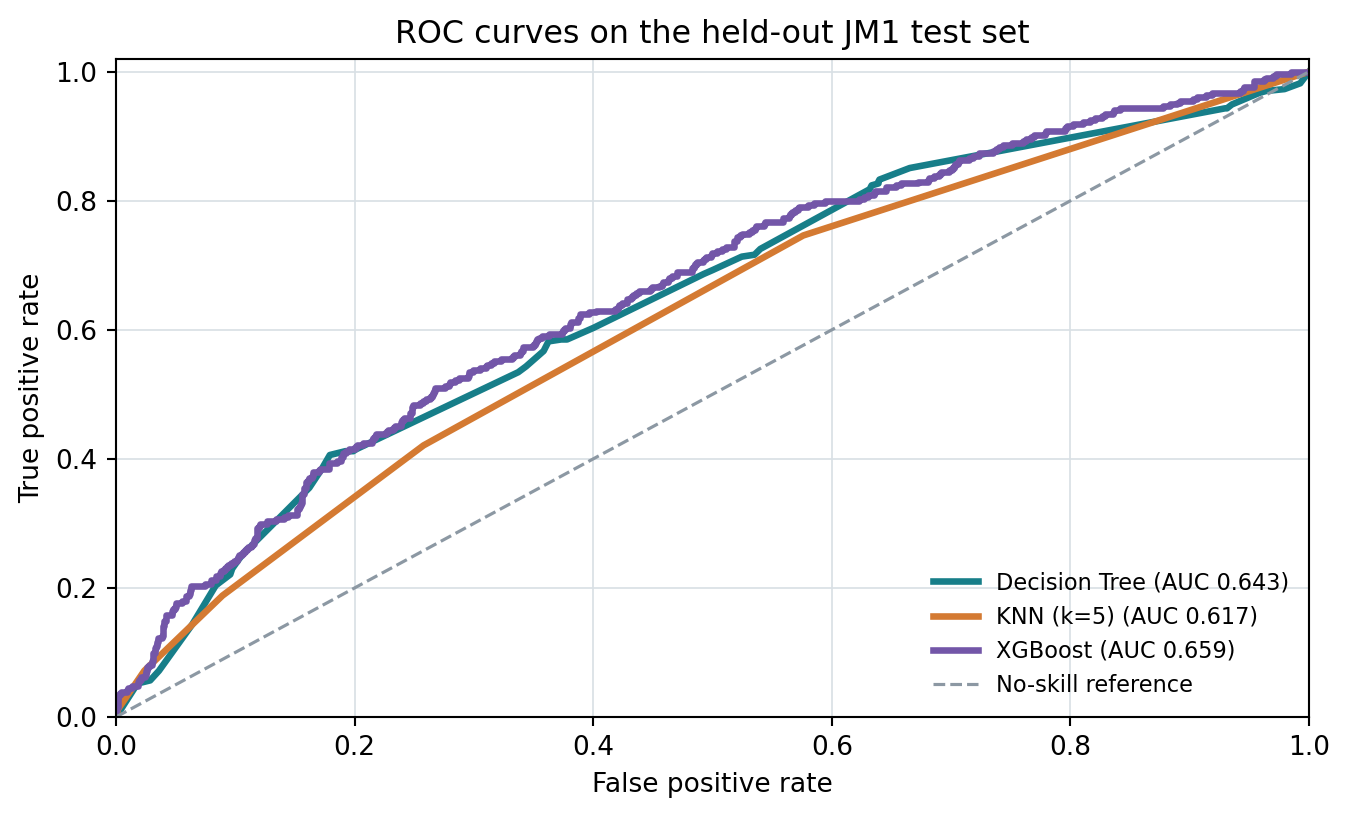
\includegraphics[width=0.78\textwidth]{figures/roc_curve.png}
\caption{ROC curves on the held-out JM1 test set.}
\label{fig:roc}
\end{figure*}

\begin{figure*}[t]
\centering
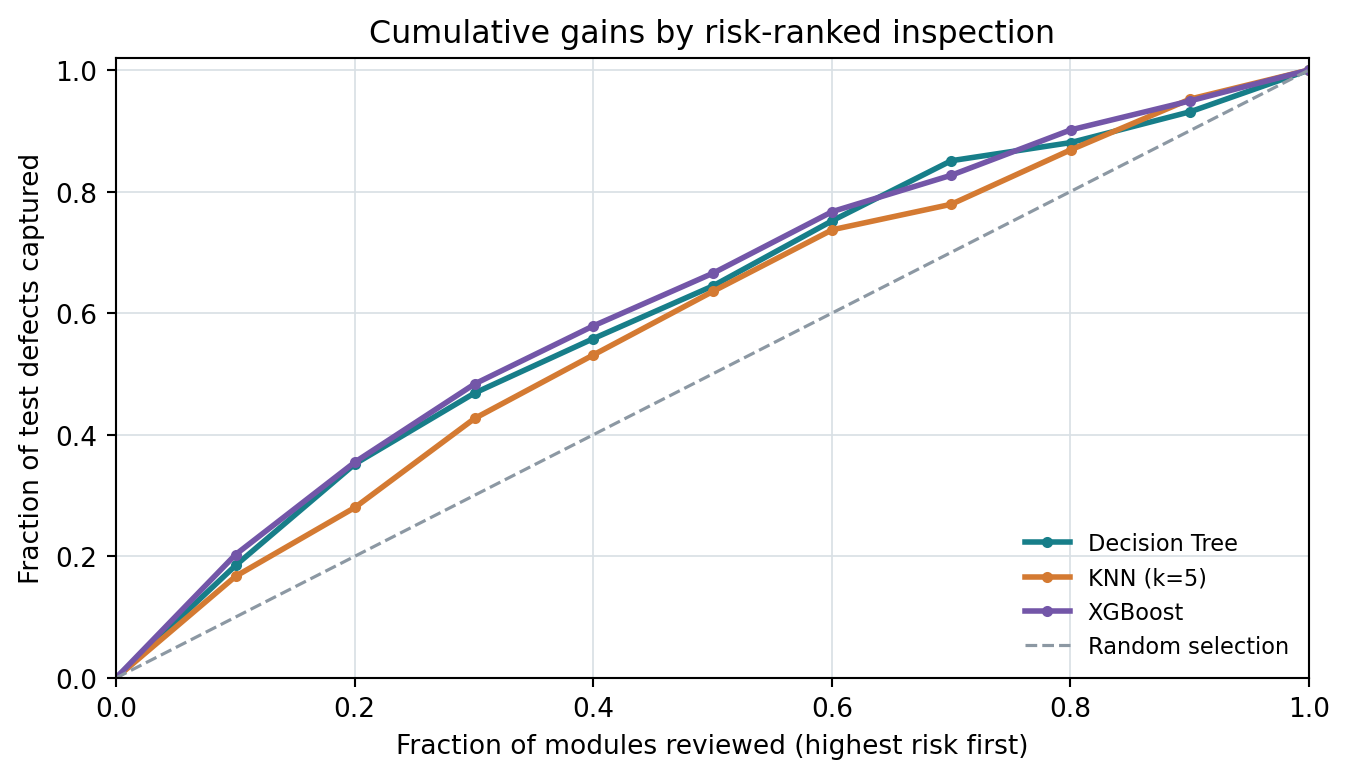
\includegraphics[width=0.78\textwidth]{figures/cumulative_gains.png}
\caption{Cumulative fraction of test defects captured by reviewing modules in descending predicted-risk order.}
\label{fig:gains}
\end{figure*}

\subsection{Feature Importance}
The Decision Tree's five leading impurity-based features were \texttt{LOC\_TOTAL} (0.394), \texttt{LOC\_BLANK} (0.122), \texttt{LOC\_EXECUTABLE} (0.088), \texttt{HALSTEAD\_EFFORT} (0.075), and \texttt{HALSTEAD\_CONTENT} (0.054). XGBoost's five leading gain-based importances were \texttt{LOC\_TOTAL} (0.103), \texttt{LOC\_BLANK} (0.078), \texttt{NUM\_UNIQUE\_OPERANDS} (0.060), \texttt{LOC\_EXECUTABLE} (0.056), and \texttt{HALSTEAD\_VOLUME} (0.050). Importance values are model-specific split summaries, not causal effects. Because metrics are correlated, importance may be divided among related features.

% Flush the Results floats before discussion, conclusion, and references.
\clearpage

\section{Discussion}
The three models present different operating trade-offs. XGBoost provides the strongest overall ranking by ROC-AUC and top-decile lift; the Decision Tree detects more defects using the default threshold. KNN's 75.5\% accuracy is below the all-non-defective baseline and coexists with low defect recall, illustrating why accuracy should not be used alone for an imbalanced target.

For limited manual review capacity, risk ranking may be more useful than a fixed default label threshold. XGBoost is the strongest candidate of these tested configurations for prioritizing the top decile, but its test-set performance is still modest. The results should be treated as educational baselines rather than evidence of production readiness.

\subsection{Limitations and Statistical Significance}
Only JM1 and one stratified holdout split were analyzed. We did not perform cross-validation, hyperparameter tuning, external validation, or a hypothesis test; no p-value or statistical superiority claim is reported. Scores are descriptive for this split and may vary across splits and projects. The benchmark labels and static metrics may not transfer to a current software team. Correlation and feature importance are not interpreted causally.

\section{Conclusion}
On this JM1 holdout, XGBoost achieved the strongest defect-risk ranking (ROC-AUC 0.659; top-decile lift 2.03), while the class-balanced Decision Tree achieved the highest default-threshold recall (56.7\%). KNN had low recall (18.8\%) and did not exceed the majority-class accuracy baseline. All models show limited predictive quality. Repeated validation, threshold selection based on review costs, and evaluation on independent projects are needed before practical use.

\section*{Reproducibility}
The split used \texttt{train\_test\_split(test\_size=0.20, stratify=y, random\_state=42)}. The analysis ran with scikit-learn 1.7.2 and XGBoost 3.4.1. All reported metrics were computed from the repository's JM1 ARFF file.

\bibliographystyle{IEEEtran}
\bibliography{references}

\end{document}
